\newsection{Casi d'uso}
\subsection{Struttura}
Ogni caso d'uso è descritto dalla seguente struttura:
\begin{itemize}
	\item codice identificativo: $$ \textbf{UC \{codice\_padre\}.\{codice\_figlio\}  } $$
	\begin{itemize}
		\item UC specifica che si tratta di un caso d'uso;
		\item codice\_padre identifica univocamente i casi d'uso;
		\item codice\_figlio è un numero progressivo che identifica i sottocasi.
	\end{itemize}
	\item titolo;
	\item diagramma UML;
	\item attori;
	\item scopo e descrizione;
	\item precondizione;
	\item flusso base degli eventi;
	\item postcondizioni;
	\item inclusioni (se presenti);
	\item estensioni (se presenti).
\end{itemize}

\newpage
\subsection{Elenco dei casi d'uso}
\begin{figure} [H]
	\centering
	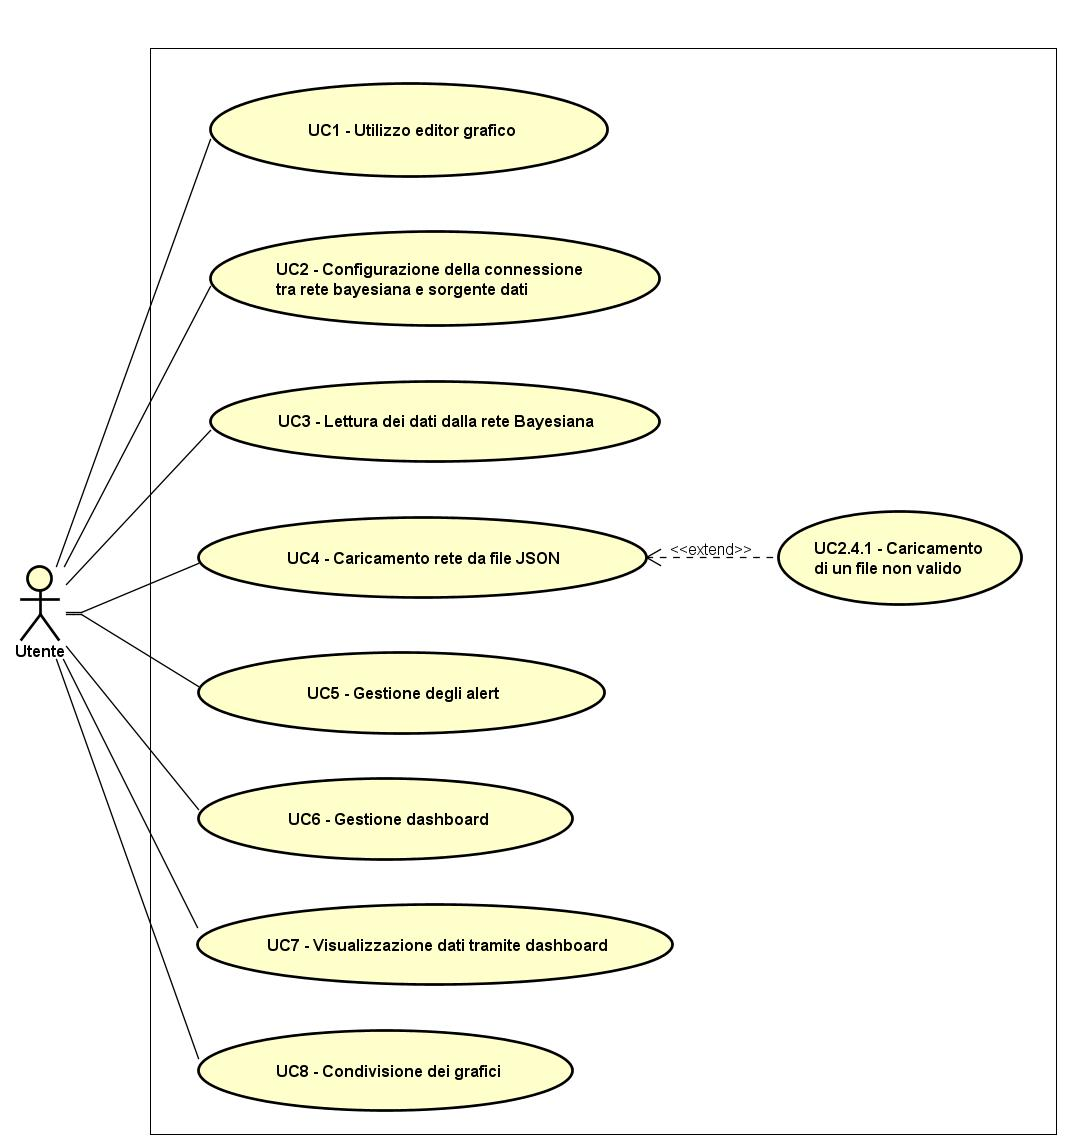
\includegraphics[scale=0.5]{Img/UC}
	\caption{Diagramma dei casi d'uso}\label{}
\end{figure}
